\documentclass{beamer}
\usepackage{beamerthemesplit}
\usepackage{amsmath}
\usepackage{adjustbox}
\usepackage{amssymb}
\usepackage{subfigure}
\usepackage{amsfonts}
\usepackage{newlfont}
\usepackage{graphics}
\usepackage{graphicx}
\usepackage{epsfig}
\usepackage{booktabs}
\usepackage{booktabs, longtable,array}


\usepackage[english]{babel}
\usepackage[latin1]{inputenc}
%\usepackage{hyperref}
%\usepackage[round]{natbib}

% \usetheme{default}
% \usetheme{Boadilla} %# not so good
% \usetheme{Madrid}  % # not so good
% \usetheme{Montpellier}
% \usetheme{Warsaw}
% \usetheme{Copenhagen}
% \usetheme{Goettingen}
% \usetheme{Hannover}
%\usetheme{Berkeley}
\usecolortheme{orchid}
\beamertemplatesolidbackgroundcolor{white!65}
\setlength{\parskip}{8pt plus 1pt minus 1pt}
\setbeamertemplate{footline}[frame number]


\title[IIT Roorkee]{LOW COST HARDWARE DESIGN FOR IOT
APPLICATION IN INDUSTRIAL PROCESS}
\author{B.Tech Project Presentation Group Number-07}
\author{Gundappa DH (2015IPG-032)\\
        Kuthadi Sanjeev Kumar (2015IPG-046)\\
        Sachin Nikunj (2015IPG-78)\\
\vspace{6mm}
\textbf{Supervised by: Dr. Presenjit Chanak}} 
\institute[]{
	
	ABV-Indian Institute of Information Technology and\\
	Management, Gwalior
}
\date{\today}


\begin{document}
	\frame{\titlepage}
	
	%\begin{frame}
	%\frametitle{Outline}
	%\tableofcontents[pausesections]
	%\end{frame}
	
	\begin{frame}\frametitle{Contents}
	\begin{itemize}
		\item	Introduction
		\item   Literature Review
		\item   Problem Statement 
		\item	Implementation  
		\item   Testing
		\item	Results
		\item   Conclusion and Future works
	\end{itemize}
\end{frame}
\begin{frame}\frametitle{}
\Huge
\begin{center}INTRODUCTION \end{center}
\end{frame}

\begin{frame}\frametitle{Internet Of Things and its Importance }
\begin{itemize}

\item	Internet Of Things
\begin{itemize}
	\item Is a network of physical objects, embedded with sensors, electronics and soft wares .	 
	\item Which enables network connectivity and helps in collecting and exchanging the data.	  
\end{itemize}
\item Importance
\begin{itemize}
	\item It can be next industrial revolution in terms of automation. 
	\item Makes easy to integrate all the objects for making the devices.
\end{itemize}
\end{itemize}
\end{frame}




\begin{frame}\frametitle{Problem statement}
\begin{figure}[h]
\centerline{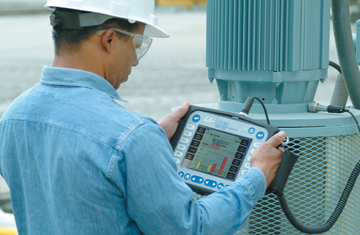
\includegraphics[width=3.7in]{health}}
\end{figure}
\end{frame}
\begin{frame}\frametitle{Implementation}
\item Major implementations of our objective 
\begin{itemize}

\item Integration of ultrasonic sensor on Arduino .
\item Integration of Sound sensor on Arduino.
\item Integration of Multiple sensor on Arduino.
\item Transmission of data  using two  Bluetooth modules .
\item Transmission of data to cloud platform.

\end{itemize}
\end{frame}
\begin{frame}\frametitle{Integration of ultrasonic senor on Arduino.}
\begin{itemize}
\item we have used ultrasonic sensor to calculate the distance of the object placed in front of the sensor.
\item .
\end{itemize}
\end{frame}

\begin{frame}\frametitle{Integration of sound sensor on Arduino}
\begin{itemize}
\item The sound sensor is used to calculate the  sound variations in the  surroundings  .  
\item   .  
\item   .
\end{itemize}
\end{frame}

\begin{frame}\frametitle{Architecture of Basic master device}
\begin{itemize}
  \begin{figure}[H]
  \centerline{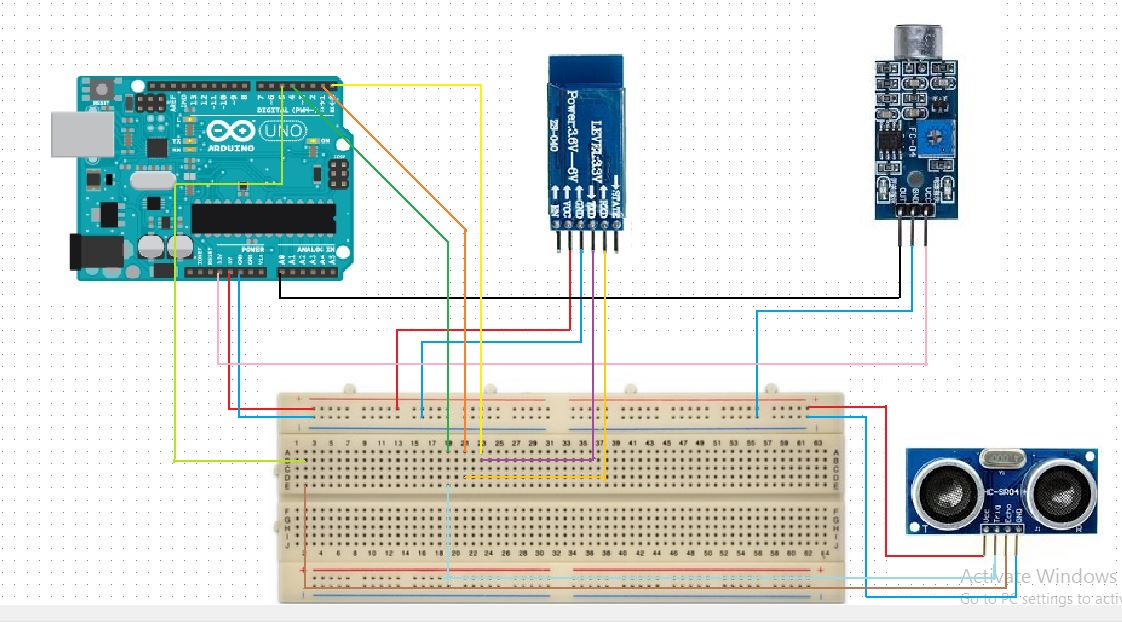
\includegraphics[width=4.0in]{master.JPG}}
  \caption{ \textbf{}Master device architecture}
  \end{figure}
\end{itemize}
\end{frame}
\begin{frame}\frametitle{Architecture of basic slave device }
\begin{itemize}
\begin{figure}[h]
\centerline{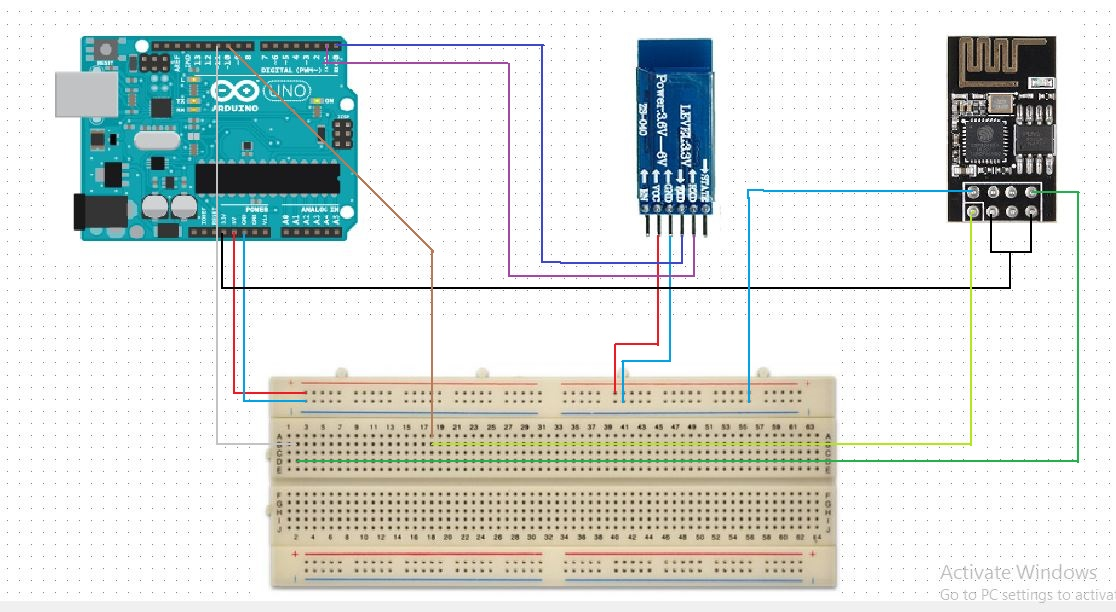
\includegraphics[width=3.7in]{slave}}
\caption{slave device architecture  .}
\end{figure}
\end{itemize}
\end{frame}
  \begin{frame}\frametitle{Integration of multiple sensors on Arduino.}
 \item Smoke  sensor
\begin{itemize}
\item Smoke sensor is used to detect a wide range of gases in the surroundings.
\item Wide range of gases include propane, butane, hydrogen etc.
\end{itemize}
 \item Vibration sensor
\begin{itemize}
    \item Vibration sensor is used to feel the vibration in the surroundings. 
\end{itemize}
.

\end{frame}
 \begin{frame}
 \item Humidity and Temperature sensor
\begin{itemize}
\item Humidity and temperature sensor is used to calculate the relative humidity in the air.
\item It is also used to calculate the change in the temperature in the surroundings.
\end{itemize}
\end{frame}

\begin{frame}\frametitle{Master device}
\begin{itemize}
  \begin{figure}[H]
  \centerline{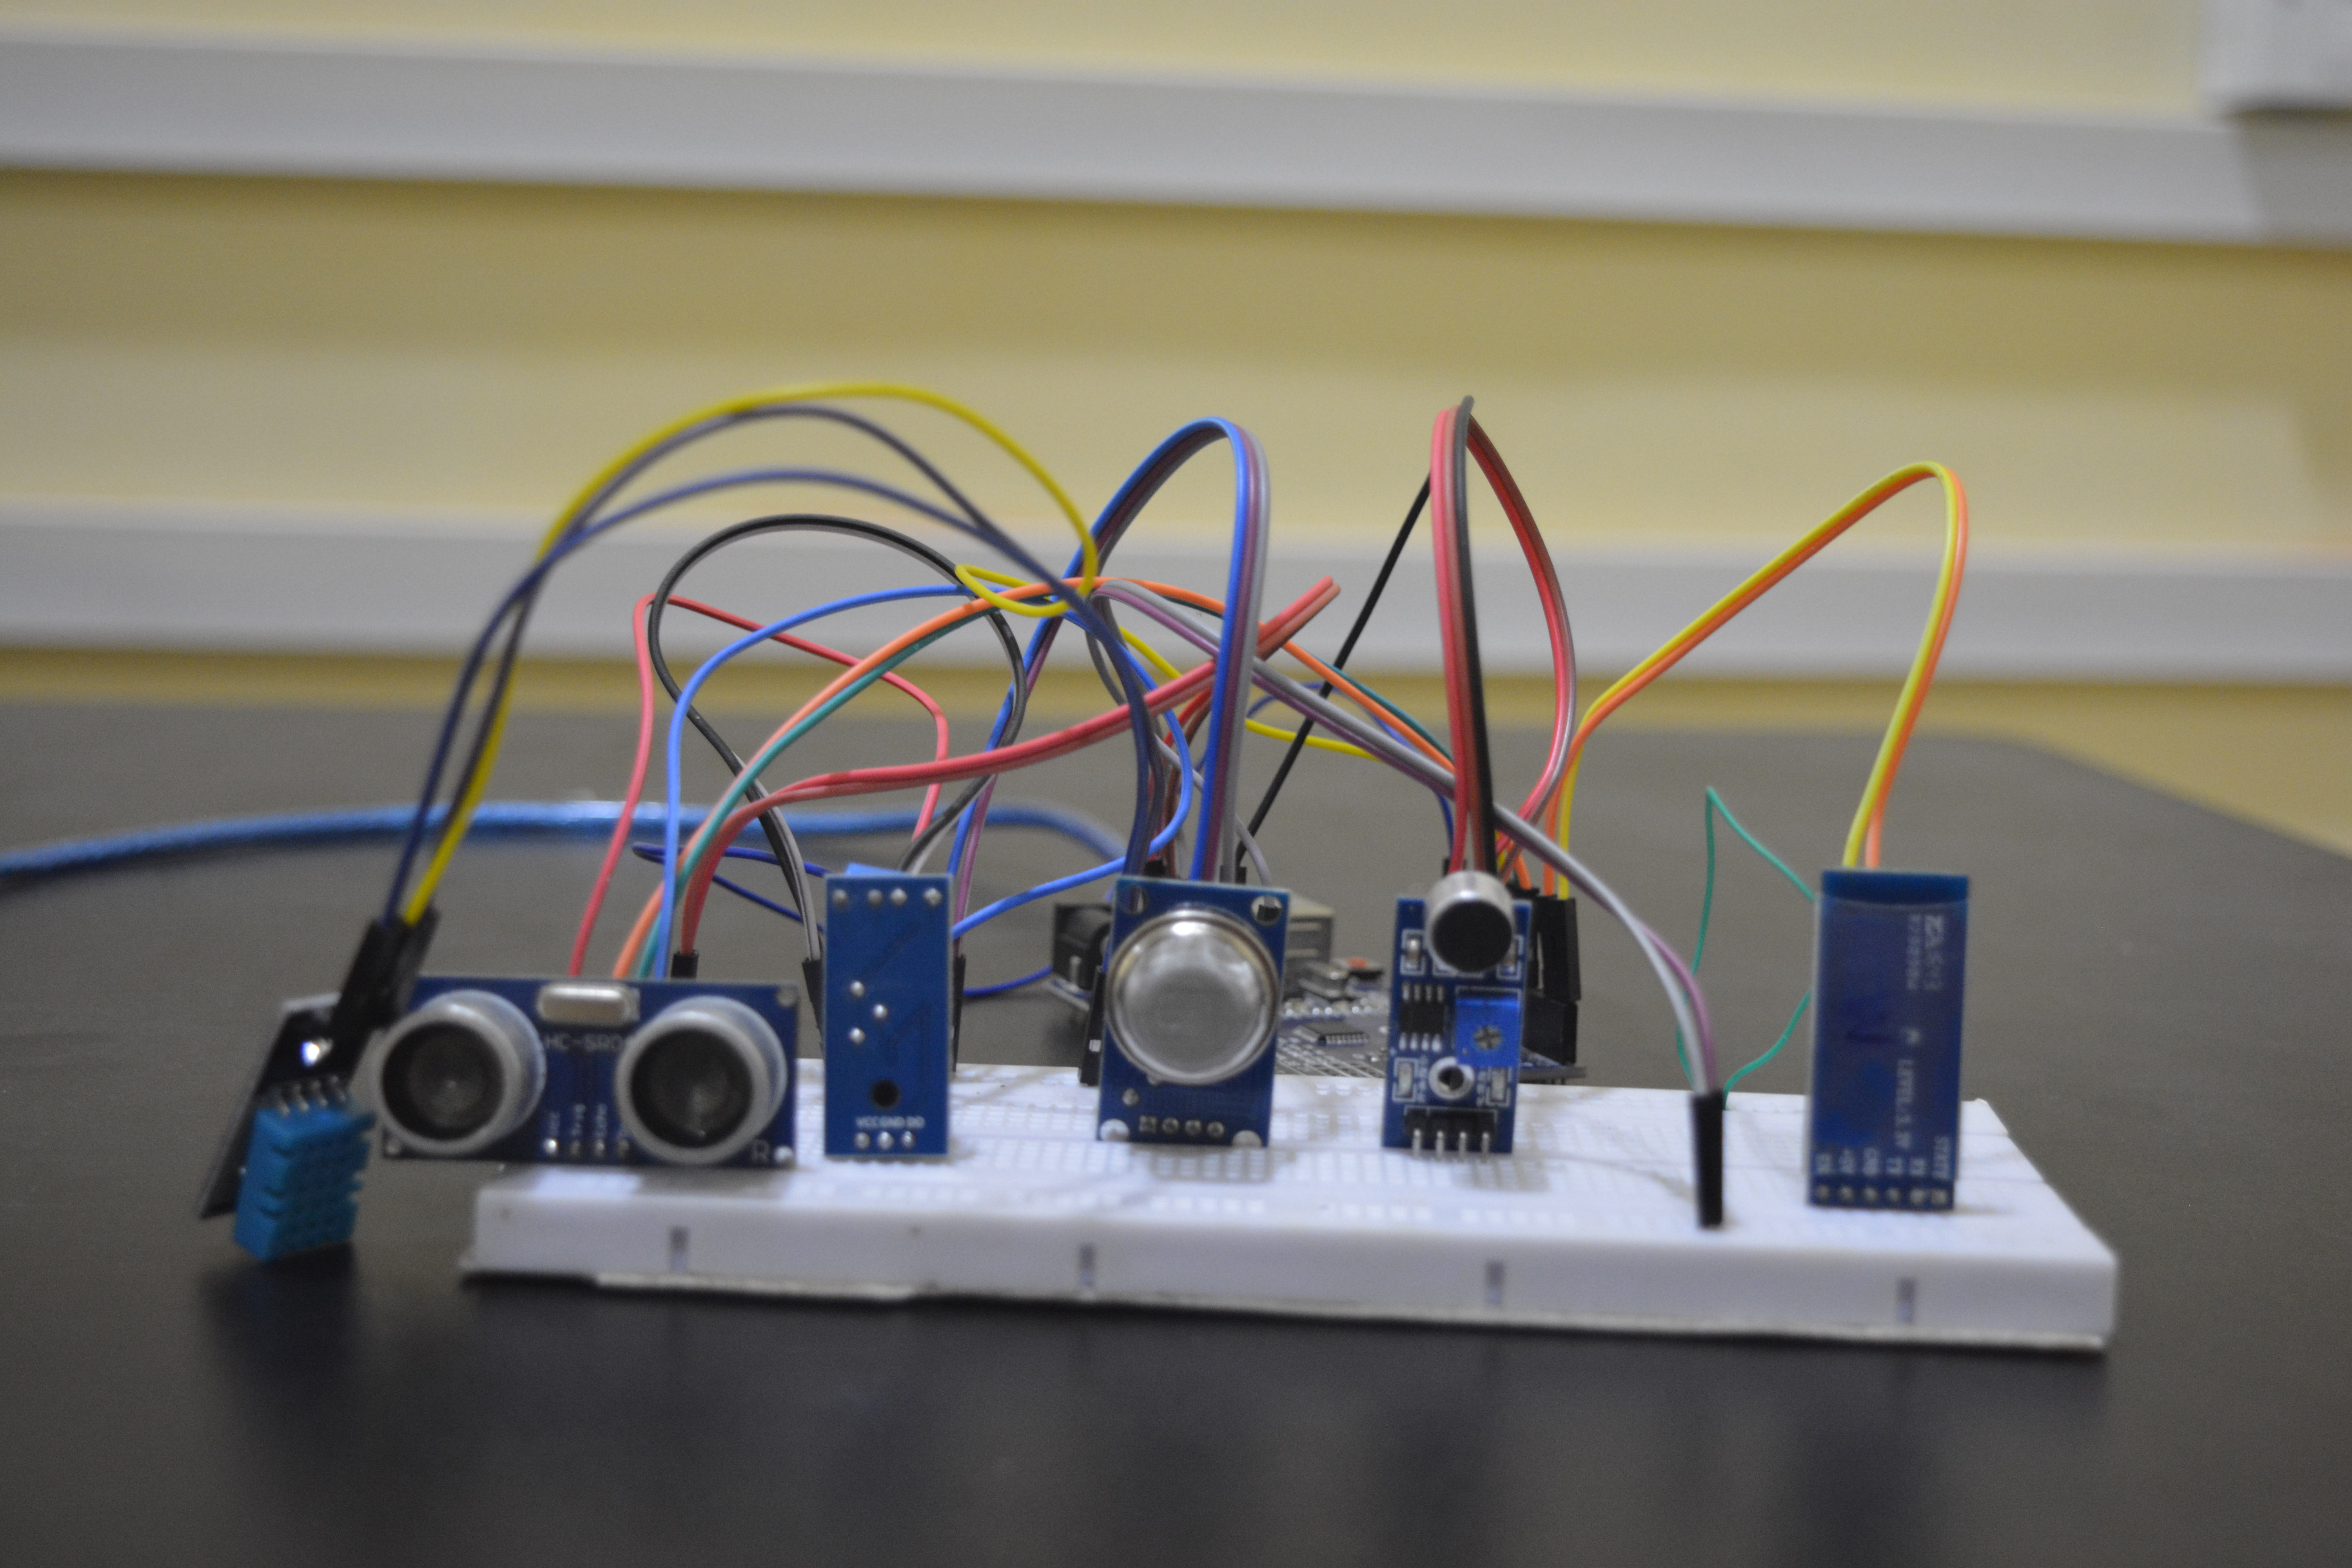
\includegraphics[width=4.0in]{master2.JPG}}
  \caption{ \textbf{}Master device to collect data from the sensors}
  \end{figure}
\end{itemize}
\end{frame}

\begin{frame}\frametitle{Slave  device}
\begin{itemize}
  \begin{figure}[H]
  \centerline{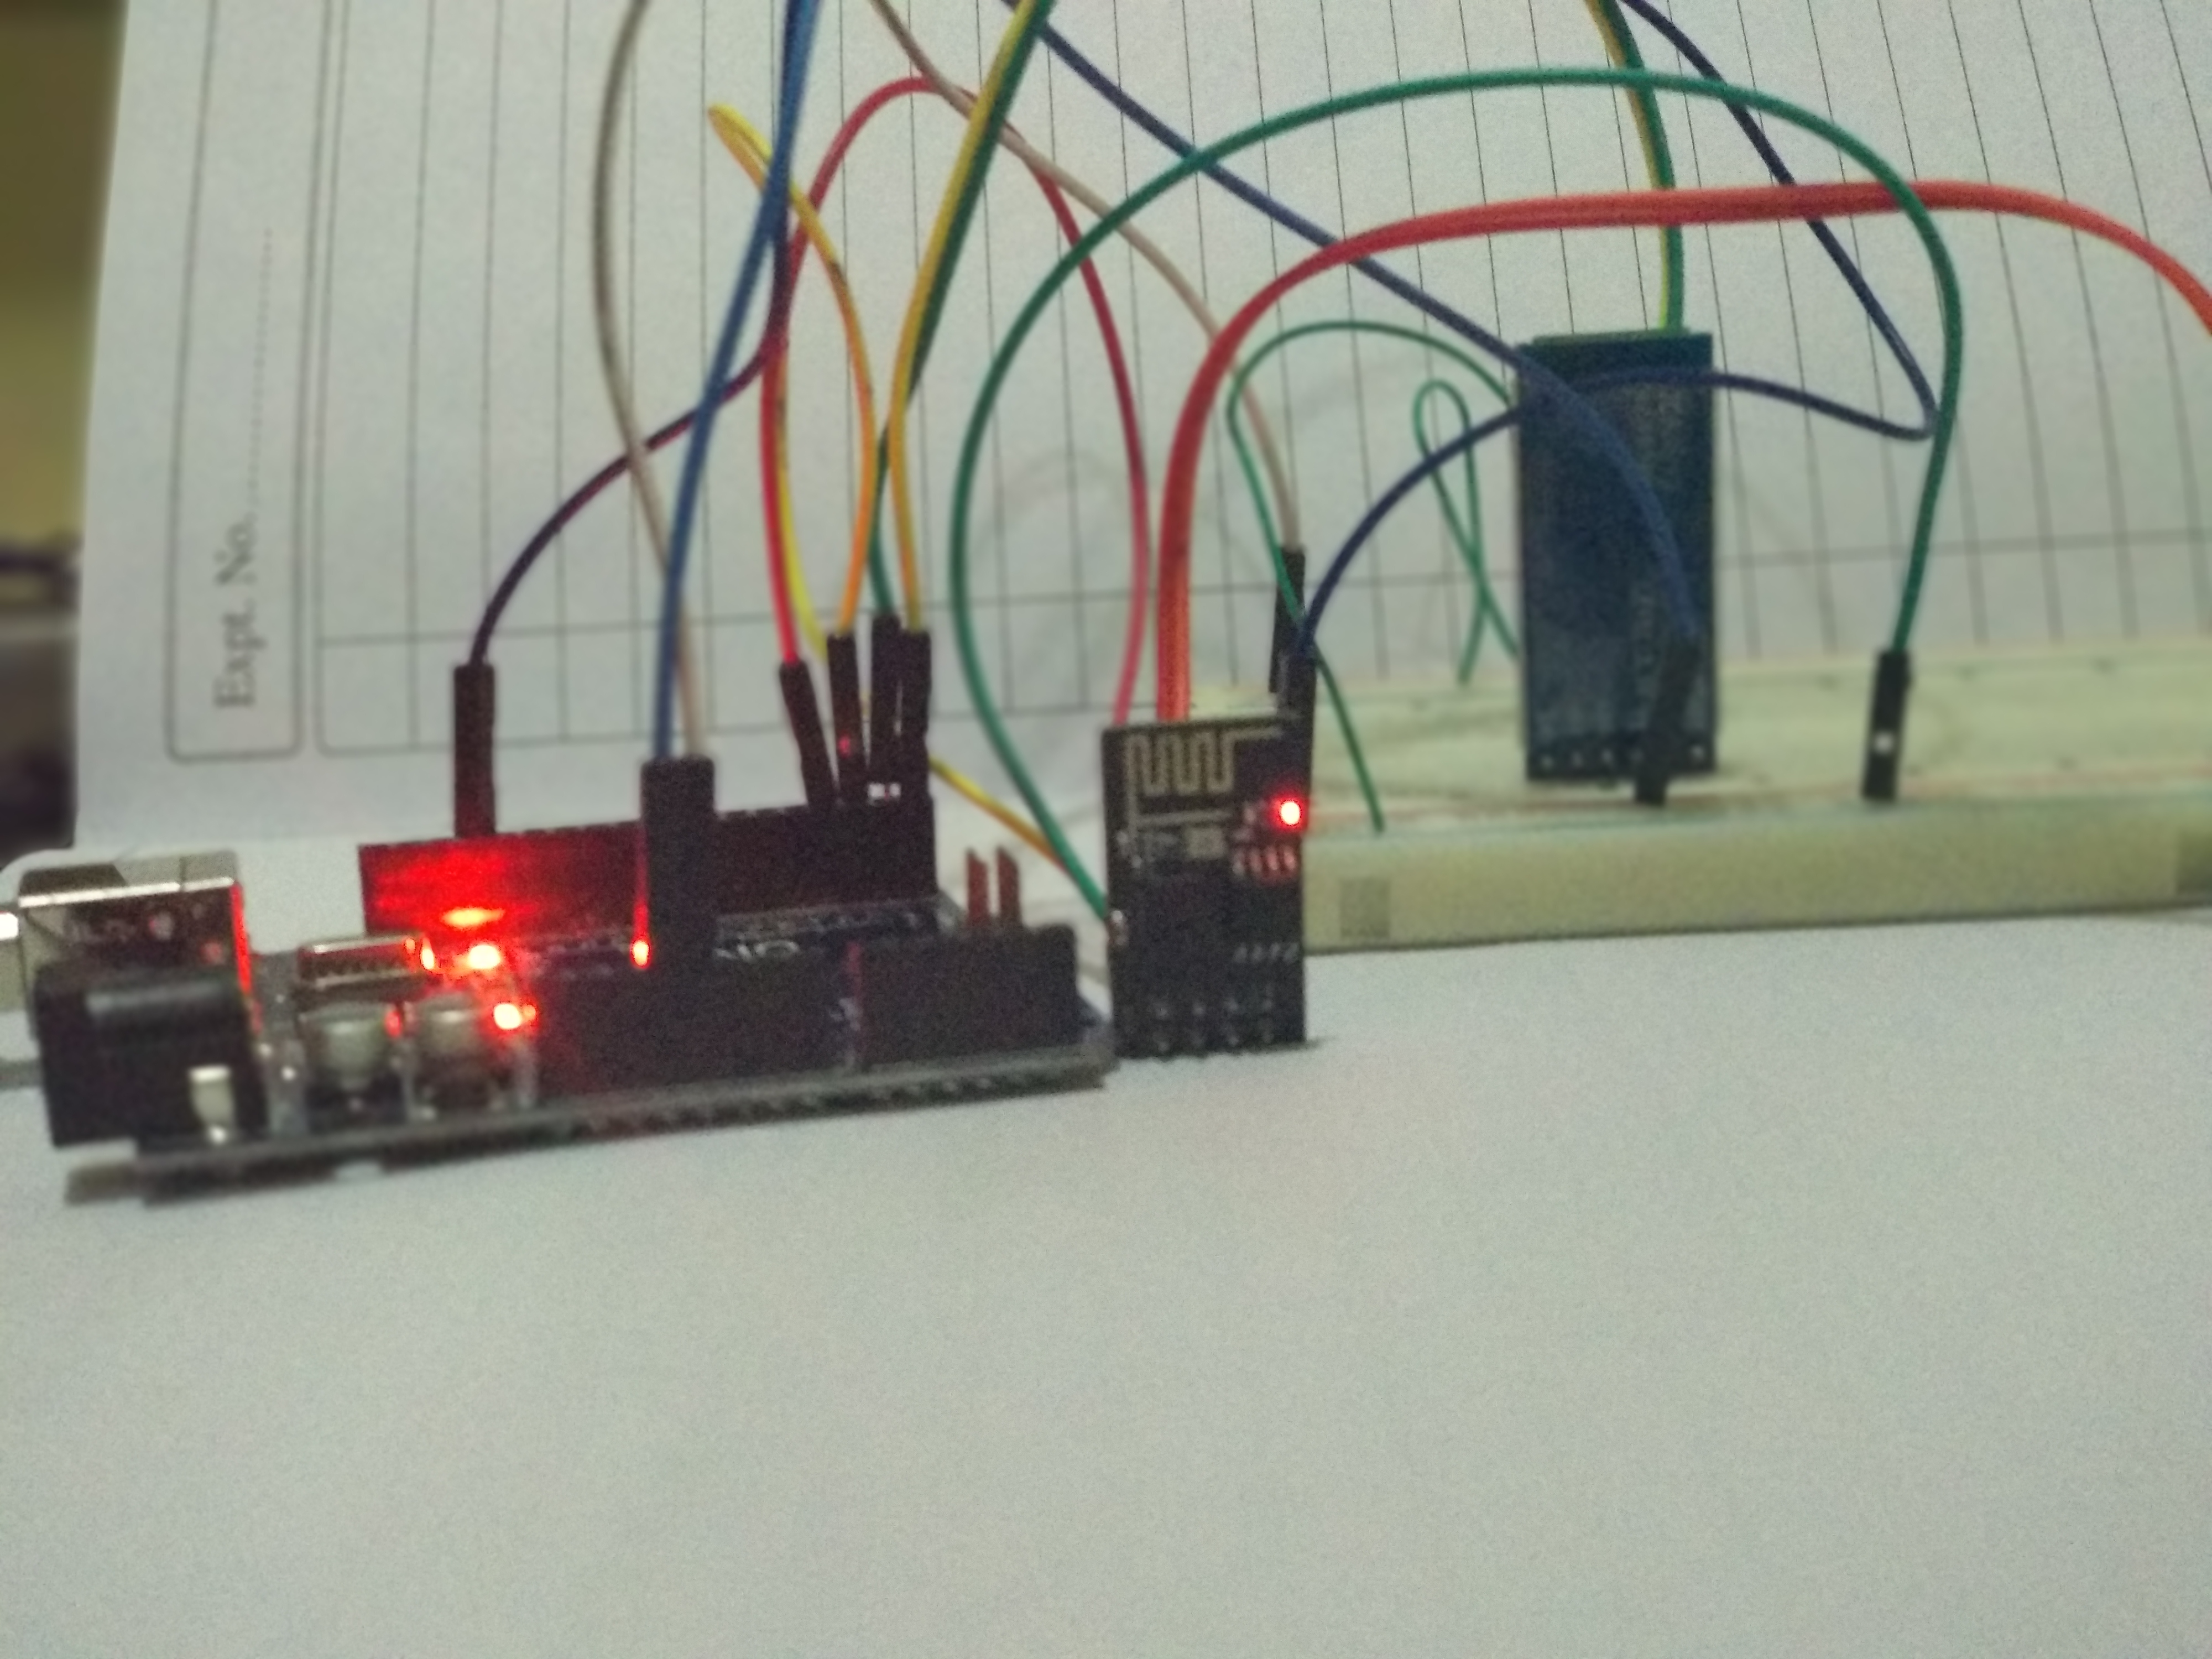
\includegraphics[width=4.0in]{slave22}}
  \caption{ \textbf{}Slave device to transfer data to the cloud}
  \end{figure}
\end{itemize}
\end{frame}
\begin{frame}\frametitle{Communication between master and slave device.}
\begin{itemize}
\item Bluetooth module is used to communicate between master and slave device.
\item A master Bluetooth module is connected to master device to send data to the slave device. 
\item A slave Bluetooth module is connected to slave device to receive data from the master device.
\item Bluetooth modules used serial port protocol for communication between two device.
\end{itemize}
\end{frame}
\begin{frame}\frametitle{Saving data into cloud.}
\begin{itemize}
\item ESP2866 WIFI module is used to send sensor data into cloud. 
\item We had used Think-Speak cloud to save our sensor data into cloud.
\end{itemize}
\end{frame}
\begin{frame}\frametitle{Testing.}
\begin{itemize}
\item We have tested few sensors on different environments.
\item We also used different set of sensors for different. requirements.  
\end{itemize}
\end{frame}
\begin{frame}
\begin{itemize}\frametitle{Results}
\item We have integrated five sensors on a single micro controller for effective reliability. 
\item We have established a wireless communication between two devices.
\item We have used different configuration of sensors for different environments.
\item The data collected is stored in a cloud storage for documentation.
\end{itemize} 
\end{frame}
\begin{frame}
\begin{itemize}
\item Data representation for ultrasonic sensor and sound sensor in cloud.
  \begin{figure}[H]
  \centerline{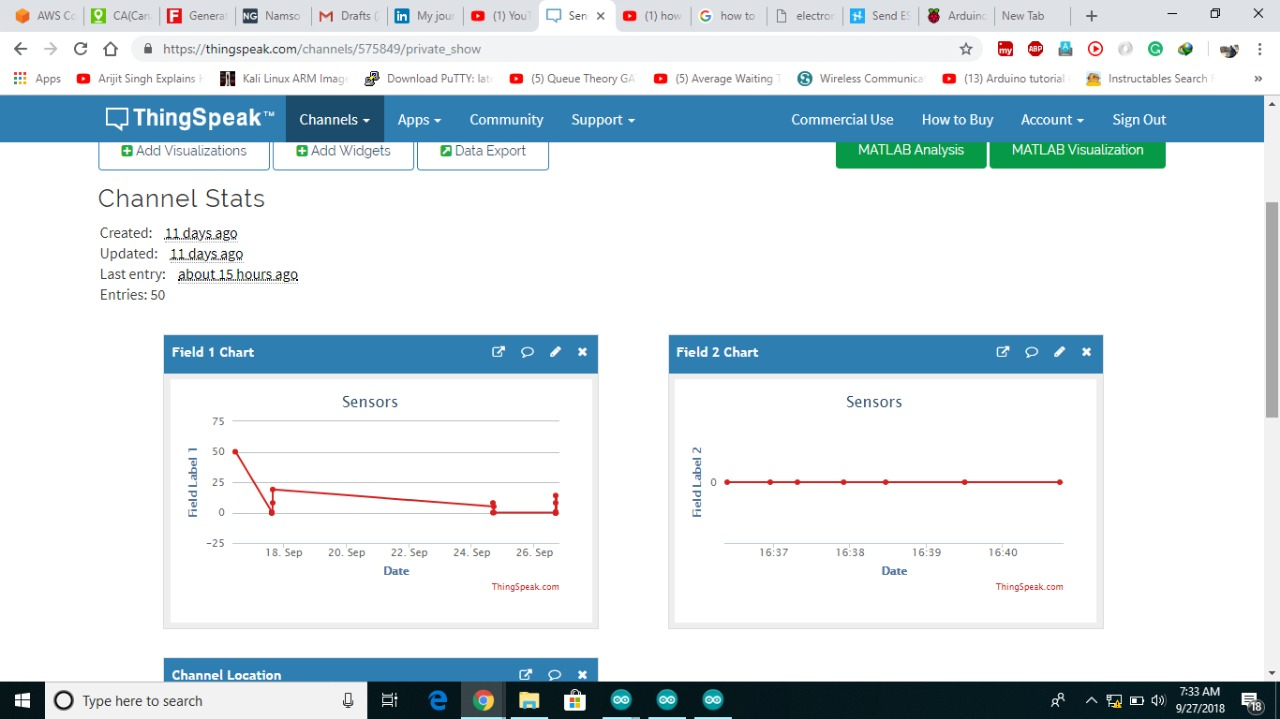
\includegraphics[width=4.0in]{two.JPG}}
  \caption{ \textbf{}Data representation in cloud for two sensors}
  \end{figure}
\end{itemize}
\end{frame}
\begin{frame}
\begin{itemize}
\item Data representation for multiple sensors in cloud.
  \begin{figure}
  \centerline{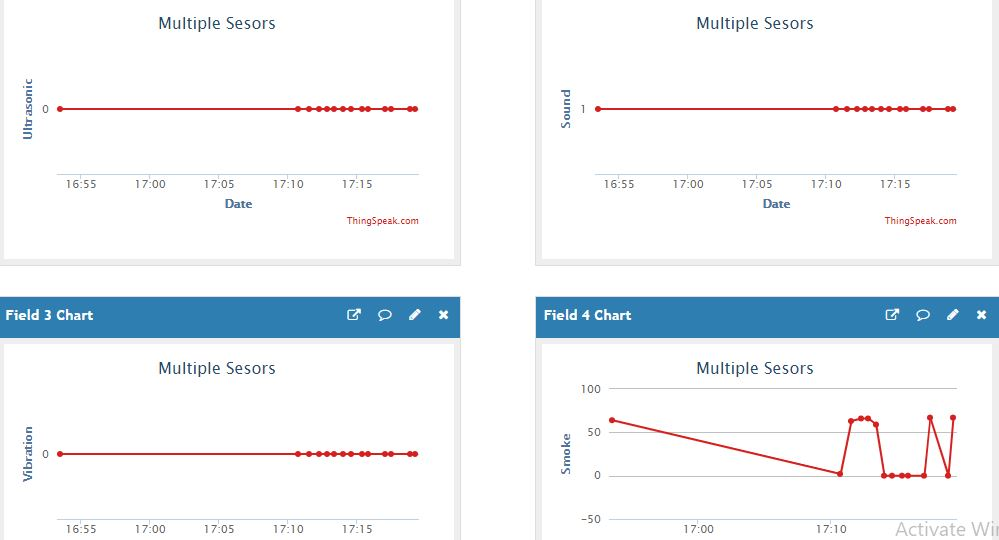
\includegraphics[width=4.0in]{multiplesensor.JPG}}
  \caption{ \textbf{}Data representation in cloud for multiple sensors}
  \end{figure}
\end{itemize}
\end{frame}

\begin{frame}\frametitle{Conclusion}
\item Numerous tampering detection techniques have been proposed before are intending to detect the tamper in a video.
\begin{itemize}
    \item Using various techniques such as watermarking, signature detection.
    \item That techniques  can  detect  only  MPEG2  encoded  videos.
\end{itemize}
\begin{itemize}
\item This algorithm detects  inter tampered frames in any kind of videos such as MPEG2 and MPEG4 encoded videos.
\end{itemize}
\end{frame}
\begin{frame}\frametitle{Future Work}
Future work may comprise
\begin{itemize}
\item As a future work we will test our project in the industries.
\item We will test and integrate different kind of sensor to adjust different environment requirements.
\end{itemize}
\end{frame}
\begin{frame}\frametitle{References}
\begin{itemize}
\newcolumntype{P}[1]{>{\raggedright\arraybackslash}p{#1}}


\begin{longtable}{P{\dimexpr0.20\textwidth-2\tabcolsep-5\arrayrulewidth\relax}
                        P{\dimexpr0.5\textwidth-4\tabcolsep-4\arrayrulewidth\relax}
                        P{\dimexpr0.5\textwidth-4\tabcolsep-4\arrayrulewidth\relax}}

\toprule
 Authors & Title & Details\\\midrule

\multicolumn{3}{c}{}\\
 Arab F, Abdullah SM, Hashim SZM, Manaf AA, Zamani M  & A robust video watermarking technique for the tamper detection of surveillance systems & It is used for different purposes including authentication and tamper detection.\\\midrule
\multicolumn{3}{c}{}\\
Tanfeng Sun, Wan Wang & Exposing video forgeries by detecting MPEG double compression & An improved video tampering detection model based on MPEG double compression is proposed.\\\midrule


\bottomrule
\end{longtable}

\end{itemize}
\end{frame}

\begin{frame}\frametitle{}
\Huge
\begin{center}Thank You \end{center}
\end{frame}



\end{document}